%==============================================================================
%  Mycellium-Aegis — Yapay Zekâ ve Sinyal Zekâsı Planı (Jüri Sunumu, TR)
%  Beamer sunumu — ayrıntılı, jüriyi ikna etmeye yönelik sürüm.
%  APA 7 yazılı plana (Mycellium-Aegis_AI_Plan_APA7.md) eşlik eder.
%
%  Derleme:  pdflatex -interaction=nonstopmode Mycellium-Aegis_YZ_Plani_Sunum_TR.tex
%            (bölüm/çerçeve sayaçları otursun diye İKİ KEZ çalıştırın)
%
%  Kendi kendine yeten: yalnızca standart TeX Live paketleri
%  (beamer, tikz, booktabs, xcolor, lmodern, microtype, appendixnumberbeamer).
%  Türkçe karakterler T1 + utf8 + lmodern ile gelir (babel-turkish gerekmez).
%==============================================================================
\PassOptionsToPackage{table}{xcolor}
\documentclass[aspectratio=169,11pt]{beamer}

\usepackage[T1]{fontenc}
\usepackage[utf8]{inputenc}
\usepackage{lmodern}
\usepackage{microtype}
\usepackage{booktabs}
\usepackage{tikz}
\usepackage{appendixnumberbeamer}
\usetikzlibrary{arrows.meta,positioning,shapes.geometric,calc}

% Türkçe tireleme yok; satır sonu esnekliğini artırıp taşmayı önleyelim
\tolerance=2500
\hbadness=2500
\emergencystretch=3em

%------------------------------------------------------------------ renkler ---
\definecolor{aegisGreen}{HTML}{2E7D32}
\definecolor{aegisDark}{HTML}{1B5E20}
\definecolor{aegisLeaf}{HTML}{4E8A3A}
\definecolor{aegisAI}{HTML}{6A1B9A}
\definecolor{aegisBlue}{HTML}{0277BD}
\definecolor{aegisInk}{HTML}{233329}
\definecolor{aegisMist}{HTML}{EAF1EA}
\definecolor{aegisAmber}{HTML}{C77800}

%------------------------------------------------------------------- tema -----
\usetheme{default}
\usecolortheme{default}
\setbeamercolor{normal text}{fg=aegisInk}
\setbeamercolor{structure}{fg=aegisGreen}
\setbeamercolor{frametitle}{fg=white,bg=aegisDark}
\setbeamercolor{title}{fg=aegisDark}
\setbeamercolor{alerted text}{fg=aegisAmber}
\setbeamercolor{block title}{fg=white,bg=aegisGreen}
\setbeamercolor{block body}{fg=aegisInk,bg=aegisMist}
\setbeamercolor{itemize item}{fg=aegisLeaf}
\setbeamercolor{itemize subitem}{fg=aegisLeaf}
\setbeamercolor{section in toc}{fg=aegisInk}

\setbeamerfont{frametitle}{series=\bfseries}
\setbeamerfont{title}{series=\bfseries,size=\LARGE}
\setbeamertemplate{navigation symbols}{}
\setbeamertemplate{itemize items}[circle]
\setbeamertemplate{blocks}[rounded][shadow=false]

% çerçeve başlığı: tam genişlik bant
\setbeamertemplate{frametitle}{%
  \nointerlineskip
  \begin{beamercolorbox}[wd=\paperwidth,ht=3.1ex,dp=1.2ex,leftskip=0.6cm,rightskip=0.6cm]{frametitle}%
    \usebeamerfont{frametitle}\insertframetitle%
  \end{beamercolorbox}%
}

% ince alt bilgi
\setbeamertemplate{footline}{%
  \leavevmode\hbox{%
    \begin{beamercolorbox}[wd=.30\paperwidth,ht=2.4ex,dp=1ex,leftskip=.3cm]{author in head/foot}%
      \color{aegisDark}\footnotesize Mycellium-Aegis%
    \end{beamercolorbox}%
    \begin{beamercolorbox}[wd=.54\paperwidth,ht=2.4ex,dp=1ex,center]{title in head/foot}%
      \color{aegisInk}\footnotesize Yapay Zekâ ve Sinyal Zekâsı Planı%
    \end{beamercolorbox}%
    \begin{beamercolorbox}[wd=.16\paperwidth,ht=2.4ex,dp=1ex,rightskip=.3cm]{date in head/foot}%
      \hfill\color{aegisDark}\footnotesize\insertframenumber\,/\,\inserttotalframenumber%
    \end{beamercolorbox}}%
}

% bölüm ayraç slaytları
\AtBeginSection[]{%
  \begin{frame}[plain]
    \centering
    \vfill
    {\color{aegisLeaf}\rule{2.2cm}{2pt}}\\[0.6em]
    {\usebeamerfont{title}\color{aegisDark}\insertsectionhead}\\[0.4em]
    {\color{aegisLeaf}\rule{2.2cm}{2pt}}
    \vfill
  \end{frame}
}

\newcommand{\src}[1]{{\scriptsize\color{aegisLeaf}#1}}
\newcommand{\soru}[1]{{\color{aegisAI}\bfseries #1}}

%------------------------------------------------------------------- üstveri --
\title{Yapay Zekâ ve Sinyal Zekâsı Planı}
\subtitle{Miselyum Biyoelektrik Aktivitesinden Tutuşma Öncesi Orman Yangını Tespiti için\\ LSTM Sensör Füzyonu Yaklaşımı}
\author{Muhammet Yağcıoğlu \and Mehmet Çetin \and Ömer Ünal \and Mahmut Can Göçlü}
\institute{Mycellium-Aegis \,·\, İzmir Yüksek Teknoloji Enstitüsü (İYTE) Teknopark\\ TÜBİTAK 1812 BİGG \,·\, Yeşil Büyüme}
\date{2026}

%==============================================================================
\begin{document}

%------------------------------------------------------------- başlık slaytı --
{%
\setbeamertemplate{footline}{}
\begin{frame}[plain]
  \vfill
  \begin{beamercolorbox}[wd=\paperwidth,sep=10pt,leftskip=0.8cm,rightskip=0.8cm]{block body}
    {\color{aegisLeaf}\footnotesize\bfseries YAŞAYAN MİSELYUM BİYOSENSÖRLERİ \,·\, TUTUŞMA ÖNCESİ ORMAN YANGINI ERKEN UYARISI}\\[0.7em]
    {\usebeamerfont{title}\color{aegisDark}\inserttitle}\\[0.5em]
    {\color{aegisInk}\insertsubtitle}
  \end{beamercolorbox}
  \vskip1.0em
  {\centering
    \color{aegisInk}\small\insertauthor\\[0.5em]
    {\footnotesize\color{aegisLeaf}\insertinstitute}\\[0.5em]
    {\footnotesize\color{aegisInk}\insertdate}\par}
  \vfill
  {\centering\scriptsize\color{aegisLeaf} APA~7 yazılı plana eşlik eden jüri sunumu \texttt{(Mycellium-Aegis\_AI\_Plan\_APA7.md)}\par}
\end{frame}
}

%------------------------------------------------------------------ içerik ----
\begin{frame}{Yol haritamız}
  \setbeamertemplate{section in toc}[sections numbered]
  \tableofcontents
\end{frame}

%==============================================================================
\section{Problem ve Fırsat}
%==============================================================================

\begin{frame}{Bugünkü erken uyarı sistemleri yangını çok geç görüyor}
  Uydular, İHA'lar, kamera kuleleri ve yer üstü sensör ağları tek bir kör noktayı
  paylaşır: yalnızca alev, ısı ışıması ya da duman \alert{oluştuktan sonra}
  tetiklenirler. O ana kadar yangın çoktan başlamıştır.
  \vskip0.5em
  \begin{center}
  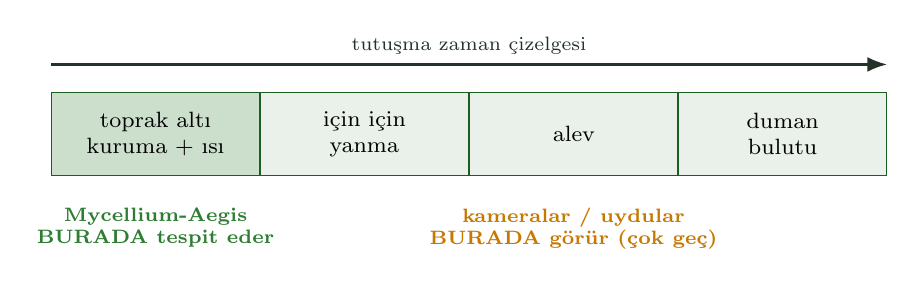
\begin{tikzpicture}[font=\footnotesize,node distance=0pt]
    \tikzset{phase/.style={draw=aegisDark,fill=aegisMist,minimum height=1.05cm,text width=2.5cm,align=center,inner sep=2pt}}
    \node[phase,fill=aegisGreen!25] (a) {toprak altı\\ kuruma + ısı};
    \node[phase,right=of a] (b) {için için\\ yanma};
    \node[phase,right=of b] (c) {alev};
    \node[phase,right=of c] (d) {duman\\ bulutu};
    \draw[-{Latex[length=2.5mm]},aegisInk,thick] ($(a.north west)+(0,0.35)$) -- ($(d.north east)+(0,0.35)$)
      node[midway,above,font=\scriptsize]{tutuşma zaman çizelgesi};
    \node[below=0.28cm of a,align=center,aegisGreen,font=\bfseries\scriptsize] {Mycellium-Aegis\\ BURADA tespit eder};
    \node[below=0.28cm of c,align=center,aegisAmber,font=\bfseries\scriptsize] {kameralar / uydular\\ BURADA görür (çok geç)};
  \end{tikzpicture}
  \end{center}
  \begin{block}{Yaklaşımın özü}
    Tespit penceresini \emph{daha erkene} — tutuşma öncesi evreye — taşıyoruz:
    yangını önceleyen toprak altı nem kaybını ve ısı birikimini izleyerek.
  \end{block}
\end{frame}

\begin{frame}{Kör nokta yapısal — ve pahalı}
  \begin{columns}[T]
    \begin{column}{0.56\textwidth}
      \textbf{Neden mevcut yığın yetersiz?}
      \begin{itemize}\small
        \item Görüş hattı, duman ve termal iz \structure{ancak yüzeyde} oluşur.
        \item Orman örtüsü altında Wi-Fi/GSM sinyali zayıflar, bataryayı tüketir.
        \item Müdahale penceresi dakikalarla ölçülür; her dakika alan ve maliyet demektir.
      \end{itemize}
      \vskip0.4em
      Yangın yalnızca bitki örtüsünü değil, toprağın fiziksel, kimyasal ve biyolojik
      yapısını da yıllarca bozar. \src{(Doerr vd., 2025)}
    \end{column}
    \begin{column}{0.44\textwidth}
      \begin{block}{Fırsat}
        Tutuşma öncesi tespit, mevcut hiçbir ticari sistemin yapısal olarak
        \emph{göremediği} bir pencereyi açar. Bu, teknik bir üstünlük \emph{ve}
        savunulabilir bir pazar konumu demektir.
      \end{block}
      \src{Hedef pazar: orman idareleri (OGM), belediyeler, enerji/altyapı hatları, sigorta.}
    \end{column}
  \end{columns}
\end{frame}

\begin{frame}{Temel fikir: orman tabanını dinlemek}
  \begin{columns}[T]
    \begin{column}{0.55\textwidth}
      Toprak altı \structure{miselyum ağları}, ısıya, kurumaya ve hasara karşı
      tekrarlanabilir, yönsel voltaj \structure{ani artışları (spike)} üretir.
      \vskip0.4em
      \textbf{15--20 cm} derinlikte $>900\,^\circ$C'lik yüzey alevi, sönümlenmiş
      $25$--$50\,^\circ$C'lik bir dalga olarak ulaşır: miselyumun hayatta kalıp
      sinyal üretmeye devam edeceği kadar serin, ama yüzeye kenetli.
      \vskip0.4em
      \src{Adamatzky (2018, 2026a, 2026b); Phillips vd.\ (2023); Doerr vd.\ (2025)}
    \end{column}
    \begin{column}{0.45\textwidth}
      \footnotesize
      \begin{tabular}{@{}r l@{}}
        \toprule
        \textbf{Derinlik} & \textbf{Biyolojik ağlara etkisi} \\
        \midrule
        0--2 cm  & neredeyse tam yıkım \\
        2--5 cm  & kısmi; sporlar hayatta \\
        5--10 cm & pirofilik mantar aktifleşir \\
        \rowcolor{aegisGreen!18}\textbf{15--20 cm} & \textbf{miselyum sensör olur} \\
        \bottomrule
      \end{tabular}
      \vskip0.4em
      \src{15--20 cm ``güvenli bölge'' hem hayatta kalınabilir hem ölçülebilir.}
    \end{column}
  \end{columns}
\end{frame}

\begin{frame}{Bu neden temelde bir \emph{Yapay Zekâ} problemi?}
  Algılama çözüldü; asıl risk \alert{karar}. Her ham kanal tek başına belirsizdir:
  \begin{itemize}
    \item sıcak bir öğleden sonra toprak sıcaklığını yükseltir,
    \item uzun bir kuraklık substrat direncini yükseltir,
    \item arka plan metabolizması ara sıra spike üretir.
  \end{itemize}
  \vskip0.3em
  \begin{block}{Sonuç}
    Tek bir kanalı naif biçimde eşiklemek, operasyonel güveni yok eden ve yangın
    söndürme kaynaklarını boşa harcayan yanlış alarmlar üretir. Yapay zekâ sistemi
    tam da bu yüzden var: zayıf, çok-hızlı sinyalleri tek bir \structure{düşük
    yanlış-alarmlı} karara dönüştürmek.
  \end{block}
\end{frame}

%==============================================================================
\section{Hedefler ve Başarı Kriterleri}
%==============================================================================

\begin{frame}{Tek bir manşet taahhüt — ve ölçülebilir}
  \begin{block}{Birincil hedef}
    Tutuşma öncesi evrede yangın başlangıcını \alert{\%1'in altında yanlış-pozitif
    oranıyla (YPO)} tespit etmek — duyarlılığı yüksek tutarak. Yüzlerce--binlerce
    düğümde yanlış alarmlar operasyonel güveni belirler.
  \end{block}
  \vskip0.2em
  \centering\footnotesize
  \begin{tabular}{@{}l l l@{}}
    \toprule
    \textbf{Hedef} & \textbf{Ölçüt} & \textbf{Kabul kriteri} \\
    \midrule
    Yanlış alarmı en aza indir & YPO & $<\%1$ (saha-temsili veride) \\
    Duyarlılığı koru           & Geri çağırma (recall) & $\ge 0{,}95$ \\
    Dengeli kalite             & PR-AUC / F$_1$ & $\ge 0{,}98$ / $\ge 0{,}95$ \\
    Zamanındalık               & Gecikme & yüzey alevinden \emph{önce} alarm \\
    Uçta uygulanabilirlik      & Model / RAM & $\le 128$ KB / $\le 256$ KB \\
    Yorumlanabilirlik          & Taban kuralla uyum & VE kuralına göre açıklanabilir \\
    \bottomrule
  \end{tabular}
  \vskip0.4em
  \src{``Saha-temsili'' = kuraklık, günlük/mevsimsel salınım ve yangın-dışı ısınmayı içerir.}
\end{frame}

\begin{frame}{Neden \%1? Ölçeğin matematiği hiçbir soru bırakmasın}
  Yanlış-pozitif oranı, filo ölçeğinde hızla \alert{büyür}. Örnek — 1000 düğüm,
  ortalama günde \emph{bir} olay-tetikli değerlendirme:
  \vskip0.3em
  \centering\footnotesize
  \begin{tabular}{@{}l l l@{}}
    \toprule
    \textbf{Model YPO} & \textbf{Günlük yanlış alarm (1000 düğüm)} & \textbf{Sonuç} \\
    \midrule
    \%5    & $\sim$50 & sistem kullanılamaz \\
    \%1    & $\sim$10 & hâlâ yorucu \\
    \rowcolor{aegisGreen!18}\%1 + uzamsal teyit & $\lesssim$1 & operasyonel olarak kabul edilebilir \\
    \bottomrule
  \end{tabular}
  \vskip0.5em
  \begin{block}{Katmanlı savunma argümanı}
    Model düzeyinde $<\%1$; ardından \structure{komşu düğüm teyidi} bağımsız
    olasılıkları çarparak ($p^k$ mertebesinde) tutarlı bir sahte kümenin
    olasılığını \emph{ondalık mertebelerce} düşürür. Etkin YPO $\ll\%1$.
  \end{block}
  \src{Varsayımlar açıkça belirtilmiştir; olay-tetikli çıkarım günlük değerlendirme sayısını zaten küçük tutar.}
\end{frame}

%==============================================================================
\section{Bilimsel Kanıt ve Veri Temeli}
%==============================================================================

\begin{frame}{Deney 1 — imza genlikte değil, \emph{frekansta}}
  \begin{columns}[T]
    \begin{column}{0.55\textwidth}
      Tek diferansiyel kanal, \emph{Pleurotus ostreatus} (istiridye mantarı),
      $f_s\approx45$ Hz, ham (GAIN\_SIXTEEN, $7{,}81\,\mu$V/bit).
      \vskip0.5em
      \footnotesize
      \begin{tabular}{@{}l r r@{}}
        \toprule
         & \textbf{Dinlenme} & \textbf{Isı stresi} \\
        \midrule
        Ortalama voltaj & $-2{,}9$ mV & $-2{,}94$ mV \\
        En düşük voltaj & $-29{,}4$ mV & $-33{,}4$ mV \\
        Baskın frekans  & $\approx20$ Hz & $\approx5$ Hz \\
        Örnek sayısı $N$ & 1.048 & 1.085 \\
        \bottomrule
      \end{tabular}
    \end{column}
    \begin{column}{0.45\textwidth}
      \begin{block}{Kilit bulgu}
        Ortalama voltaj neredeyse değişmez — ama \structure{baskın bant ısı
        stresiyle $\approx20\to\approx5$ Hz'e kayar}.
      \end{block}
      Naif bir genlik eşiği başarısız olur; \emph{spektral} ve \emph{dağılımsal}
      değişim sinyali taşır $\Rightarrow$ dizi / spektro-temporal modelleme gerekir.
    \end{column}
  \end{columns}
\end{frame}

\begin{frame}{Deney 1 — bunun modelleme için anlamı}
  \begin{itemize}
    \item Isı stresi, hücre zarındaki \structure{iyon kanalı aktivitesini} artırır;
      baskın bandı $\approx20$ Hz'den $\approx5$ Hz'e taşır.
    \item Bu, rastgele bir gürültü değil, \structure{öğrenilebilir zamansal-frekans
      yapısıdır} — tam olarak yinelemeli/spektro-temporal bir modelin yakalamak için
      tasarlandığı türden.
    \item Ortalamanın sabit kalması, \alert{sabit-seviye tespitin neden
      yetmeyeceğini} kanıtlar: karar, sinyalin \emph{şekline} ve \emph{evrimine}
      bakmalıdır.
  \end{itemize}
  \begin{block}{Jüriye net mesaj}
    Kurucu hipotez — ``miselyum, ısı stresine ayırt edilebilir biyoelektrik bir
    yanıt verir'' — projenin \emph{kendi} laboratuvar kaydıyla doğrulanmıştır. Bu,
    TRL 3$\to$4 kanıtıdır.
  \end{block}
\end{frame}

\begin{frame}{Deney 2 — sahaya doğru gerçekçilik}
  Aktif toprak--miselyum ağı, iki kanal, gerçek sayısal sinyal işleme (DSP) ile.
  \vskip0.4em
  \centering\footnotesize
  \begin{tabular}{@{}l l l@{}}
    \toprule
    \textbf{Parametre} & \textbf{Deney 1} & \textbf{Deney 2} \\
    \midrule
    Denek        & tek mantar dokusu & aktif toprak/miselyum ağı \\
    Kanal        & 1 diferansiyel & \textbf{2 diferansiyel} (ağ haritalama) \\
    PGA kazancı  & $\pm0{,}256$ V & $\pm6{,}144$ V (24$\times$ aralık) \\
    Örnekleme    & $\approx45$ Hz & $\approx100$ Hz (Nyquist 50 Hz) \\
    Filtreleme   & yok (ham) & 5-uçlu doğrusal-fazlı FIR $[0{,}1;0{,}2;0{,}4;0{,}2;0{,}1]$ \\
    Ofset kalib. & yok & otomatik (50-örnekli taban) \\
    \bottomrule
  \end{tabular}
  \vskip0.5em
  \begin{columns}[T]
    \begin{column}{0.5\textwidth}
      \src{Geniş PGA aralığı, Deney 1'i doyuran toprak--elektrot DC ofsetini ve
      empedans salınımlarını soğurur.}
    \end{column}
    \begin{column}{0.5\textwidth}
      \src{İki kanal, tek noktayı değil, ısı stresinin \emph{ağ boyunca yayılımını}
      haritalar.}
    \end{column}
  \end{columns}
\end{frame}

\begin{frame}{Deney 2 — sinyal işleme yükseltmeleri (matematik)}
  \begin{block}{Doğrusal-fazlı FIR gürültü giderme}
    \[ y[n]=0{,}1\,x[n{-}4]+0{,}2\,x[n{-}3]+0{,}4\,x[n{-}2]+0{,}2\,x[n{-}1]+0{,}1\,x[n] \]
    \small Birim DC kazancı ($\textstyle\sum_k h_k = 1{,}0$) ve doğrusal faz:
    dalga biçimini \emph{bozmadan} çevresel ve elektromanyetik gürültüyü bastırır —
    güvenilir türev öznitelikleri için önkoşul.
  \end{block}
  \begin{block}{Otomatik ofset kalibrasyonu}
    \[ V \leftarrow V - \frac{1}{50}\sum_{i=1}^{50} V_i \qquad (f_s/2 = 50\text{ Hz Nyquist, } 5\text{ Hz aksiyon potansiyellerini kapsar}) \]
    \small 50-örnekli taban çizgisi, elektrot--substrat DC bileşenini kaldırır.
  \end{block}
\end{frame}

\begin{frame}{Veri etiketleme: dört fiziksel rejim}
  \begin{columns}[T]
    \begin{column}{0.52\textwidth}
      Alarm/alarm-yok değil, \textbf{rejim düzeyinde} etiketleme:
      \begin{itemize}
        \item \structure{normal} — günlük/mevsimsel taban
        \item \structure{kuraklık} — yavaş kuruma, ısı girişi yok
        \item \structure{yangın-dışı ısınma} — güneşlenme / toprak altı kaynak
        \item \alert{yangın başlangıcı} — ısı $+$ hızlı kuruma $+$ spike birlikte
      \end{itemize}
      Modelin \emph{kuraklık ile yangını ayırt etmesini} sağlayan tam olarak budur.
    \end{column}
    \begin{column}{0.48\textwidth}
      \textbf{Kaynak ve izlenebilirlik}
      \begin{itemize}\small
        \item her kayıt tam bağlamıyla sürümlenir (tür/substrat, elektrot, kazanç,
          örnekleme, filtre, sıcaklık/nem, uyaran)
        \item ham sayımlar kalibre mV ile birlikte saklanır (yeniden kalibrasyon)
      \end{itemize}
      \src{Veri sayfası (datasheet) disiplini — Gebru vd.\ (2021).}
    \end{column}
  \end{columns}
\end{frame}

\begin{frame}{Sınıf dengesizliği ve veri artırma}
  Yangın başlangıcı, doğası gereği çok nadirdir; veri seti ağır dengesizdir. Üç
  düzeyde ele alınır:
  \begin{enumerate}
    \item \structure{Toplama} — iklim odası ve saha kampanyalarında kontrollü
      başlangıç olaylarını kasıtlı olarak fazla örnekle.
    \item \structure{Yeniden örnekleme} — öznitelik uzayında azınlık fazla-örnekleme
      (SMOTE), \alert{yalnızca eğitim bölümünde} (sızıntıyı önlemek için).
    \item \structure{Fizik-temelli artırma} — zaman bükme, ölçülen elektrot-gürültü
      sınırlarında genlik titremesi, taban çizgisi kayması enjeksiyonu, kayıtlı
      çevresel gürültü süperpozisyonu.
  \end{enumerate}
  \begin{block}{İlke}
    Artırma \emph{asla} doğrulama/test verisine uygulanmaz. Üretilen başlangıç
    örnekleri \emph{fiziksel olarak makul} kalır.
  \end{block}
  \src{SMOTE: Chawla vd.\ (2002).}
\end{frame}

%==============================================================================
\section{Yöntem ve Karar Sistemi}
%==============================================================================

\begin{frame}{Sinyal işleme ve öznitelik hattı}
  \centering
  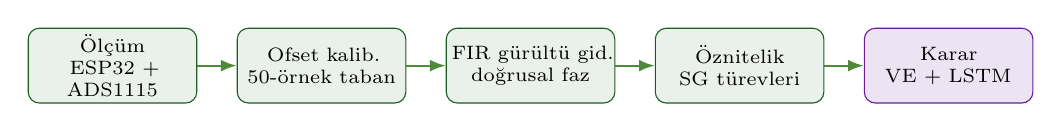
\begin{tikzpicture}[font=\scriptsize,node distance=0.42cm and 0.5cm,
      box/.style={draw=aegisDark,fill=aegisMist,rounded corners,minimum height=0.95cm,text width=2.0cm,align=center,inner sep=2pt},
      ai/.style={draw=aegisAI,fill=aegisAI!12,rounded corners,minimum height=0.95cm,text width=2.0cm,align=center,inner sep=2pt}]
    \node[box] (acq) {Ölçüm\\ ESP32 + ADS1115};
    \node[box,right=of acq] (off) {Ofset kalib.\\ 50-örnek taban};
    \node[box,right=of off] (fir) {FIR gürültü gid.\\ doğrusal faz};
    \node[box,right=of fir] (feat) {Öznitelik\\ SG türevleri};
    \node[ai,right=of feat] (dec) {Karar\\ VE $+$ LSTM};
    \foreach \a/\b in {acq/off,off/fir,fir/feat,feat/dec}
      \draw[-{Latex[length=2mm]},aegisLeaf,thick] (\a) -- (\b);
  \end{tikzpicture}
  \vskip0.6em
  \begin{columns}[T]
    \begin{column}{0.5\textwidth}
      \textbf{Çekirdek füzyon öznitelikleri}
      \begin{itemize}\footnotesize
        \item ısı akısı hızı \; $dT/dt$
        \item kuruma hızı \; $d(\ln R)/dt$
        \item spike frekansı \; $f_{\text{spike}}$
      \end{itemize}
    \end{column}
    \begin{column}{0.5\textwidth}
      \textbf{Spektral \& istatistiksel}
      \begin{itemize}\footnotesize
        \item bant-güç oranı, spektral merkez, baskın frekans
        \item varyans, çarpıklık, basıklık, Hjorth
      \end{itemize}
    \end{column}
  \end{columns}
  \vskip0.2em
  \src{Savitzky--Golay (1964) sinyali \emph{ve} türevini tek geçişte düzgünleştirir.}
\end{frame}

\begin{frame}{İki katmanlı karar sistemi}
  \begin{columns}[T]
    \begin{column}{0.5\textwidth}
      \begin{block}{1. Katman — deterministik (güvenlik tabanı)}
        \small
        \[ \text{Alarm}=(dT/dt>\beta)\ \wedge\ (d(\ln R)/dt>\gamma)\ \wedge\ \text{spike} \]
        Yorumlanabilir, neredeyse sıfır işlem, her zaman erişilebilir.
        $\beta,\gamma$ iklim odasında \textbf{\%98} güvenle sabitlenir.
      \end{block}
    \end{column}
    \begin{column}{0.5\textwidth}
      \begin{block}{2. Katman — öğrenen (LSTM)}
        \small
        Katı VE kuralının göz ardı ettiği \emph{ortak zamansal şekli} öğrenir;
        \structure{ayarlanabilir çalışma noktasıyla} YPO $<\%1$ için kalibre
        olasılık üretir.
      \end{block}
    \end{column}
  \end{columns}
  \vskip0.4em
  \begin{block}{Yükseltme (eskalasyon) mantığı}
    Yüksek önem dereceli alarm = LSTM olasılığı eşiği aşar \alert{VE} deterministik
    kural doğrular \alert{VE} komşu düğümler uyuşur. Yorumlanabilir kural döngüde
    kalır; model yanlış alarmları eler.
  \end{block}
\end{frame}

\begin{frame}{Model mimarisi — neden yinelemeli (recurrent)?}
  Yangın başlangıcı, $dT/dt$, $d(\ln R)/dt$ ve spike dinamiklerinin saniyeler--dakikalar
  boyunca \emph{birlikte evrimiyle} ve spektral göçle tanımlanır. LSTM'ler, kaybolan
  gradyan sorununu hafifleterek zamansal bağımlılıkları öğrenir
  \src{(Hochreiter \& Schmidhuber, 1997)}.
  \vskip0.4em
  \textbf{Referans model (uç-bütçesine göre boyutlanmış)}
  \begin{itemize}\small
    \item \textbf{Girdi:} pencerelenmiş öznitelik vektörü (füzyon + spektral + istatistiksel); isteğe bağlı ham kanallar.
    \item \textbf{Çekirdek:} 1--2 LSTM katmanı, 32--64 birim; küçük-veri rejimini dropout düzenler.
    \item \textbf{Baş:} 4-yönlü softmax (normal / kuraklık / yangın-dışı ısınma / yangın başlangıcı).
    \item \textbf{Kalibrasyon:} sıcaklık ölçekleme $\Rightarrow$ eşik, YPO'yu kontrol eder.
  \end{itemize}
  \src{En yüksek doğruluk için değil, ESP32 bütçesine göre boyutlandırılır.}
\end{frame}

\begin{frame}{LSTM bir başlangıç noktası — kesin sonuç değil}
  \centering\footnotesize
  \begin{tabular}{@{}l l l@{}}
    \toprule
    \textbf{Model ailesi} & \textbf{Güçlü yanı} & \textbf{Risk / uygunluk} \\
    \midrule
    \rowcolor{aegisAI!12}\textbf{LSTM} (taban) & uzun-erimli zamansal & sıralı; birincil seçim \\
    1B CNN & ucuz, spektral motif öğrenir & zayıf uzun bellek; güçlü ön uç \\
    CNN--LSTM melez & motif $+$ evrim & daha büyük; biri yetersizse \\
    TCN & uzun alım alanı, paralel & yeni MCU dışa aktarımı (Bai vd., 2018) \\
    Transformer & küresel bağlam & veri-aç; ertelendi (Vaswani vd., 2017) \\
    Gradyan artırmalı ağaçlar & sağlam tablo tabanı & doğal zamansal model yok \\
    \bottomrule
  \end{tabular}
  \vskip0.5em
  \begin{block}{Seçim kuralı}
    Hedeflere \structure{en düşük uç maliyetle} ulaşan kazanır; yorumlanabilirlik
    eşitlik bozar. Tüm öğrenen modeller, deterministik kurala \emph{ve} gradyan
    artırmalı ağaç tabanına karşı kıyaslanır — katma değer varsayılmaz, ölçülür.
  \end{block}
\end{frame}

\begin{frame}{Eğitim metodolojisi}
  \begin{columns}[T]
    \begin{column}{0.5\textwidth}
      \textbf{Dürüst bölmeler}
      \begin{itemize}\small
        \item gruplu, zaman-bloklu çapraz doğrulama
        \item birini-dışarıda-bırak: oturum (lab), saha (alan)
        \item hiçbir pencere bir bölmeyi \emph{aşmaz} $\Rightarrow$ sızıntı yok
      \end{itemize}
      \vskip0.3em
      \textbf{Dengesizlik}
      \begin{itemize}\small
        \item sınıf-ağırlıklı / odak (focal) kayıp (Lin vd., 2017)
        \item SMOTE yalnızca eğitim bölümünde (Chawla vd., 2002)
      \end{itemize}
    \end{column}
    \begin{column}{0.5\textwidth}
      \textbf{Optimizasyon}
      \begin{itemize}\small
        \item Adam (Kingma \& Ba, 2015)
        \item dropout (Srivastava vd., 2014), ağırlık sönümü, gradyan kırpma
        \item doğrulama \structure{PR-AUC}'ta erken durdurma
      \end{itemize}
      \vskip0.3em
      \begin{block}{$<\%1$ kısıtı}
        \small \emph{Eşik seçim} anında uygulanır: doğrulamada YPO $<\%1$ tutan,
        geri çağırmayı maksimize eden çalışma noktasını seç, dondur, sonra testte
        \emph{bir kez} değerlendir.
      \end{block}
    \end{column}
  \end{columns}
\end{frame}

\begin{frame}{Değerlendirme ve doğrulama merdiveni}
  \begin{columns}[T]
    \begin{column}{0.5\textwidth}
      \textbf{Ölçütler} (dengesizliğe duyarlı)
      \begin{itemize}\small
        \item YPO (birincil kısıt), geri çağırma, kesinlik, F$_1$
        \item PR-AUC (manşet), ROC-AUC
        \item yakma olayı başına tespit gecikmesi
        \item \alert{rejim ve karıştırıcı başına raporlanır}
      \end{itemize}
      \src{Aşırı dengesizlikte doğruluk (accuracy) anlamsızdır.}
    \end{column}
    \begin{column}{0.5\textwidth}
      \textbf{Doğrulama basamakları}
      \begin{enumerate}\small
        \item \structure{Lab} (İP-2): iklim odası, radyant şok; $\beta,\gamma$ sabitle.
        \item \structure{Saha} (İP-4): gömülü düğümler, kontrollü yakma — alevden \emph{önce} alarm.
        \item \structure{Uzamsal}: LoRa üzerinden komşu teyidi idiyosinkratik YPO'ları bastırır.
      \end{enumerate}
    \end{column}
  \end{columns}
\end{frame}

\begin{frame}{Yanlış alarmı nasıl \%1'in altına indiriyoruz? (7 katman)}
  \small
  Jürinin en kritik sorusu. Cevabımız tek bir hile değil, \structure{yedi bağımsız savunma}:
  \begin{enumerate}\small
    \item \textbf{Mutlak değil, hız-temelli eşikler} — mevsimsel/günlük salınıma bağışık ($dT/dt$, $d(\ln R)/dt$).
    \item \textbf{Üç-sinyal VE füzyonu} — doğal kuraklık veya sıcak gün üçünü aynı anda tetikleyemez.
    \item \textbf{Dört-rejim sınıflandırma} — kuraklığı yangından açıkça ayırır.
    \item \textbf{Doğrulamada eşik seçimi} — kalibre olasılıkta YPO $<\%1$'e sabitlenir.
    \item \textbf{Olasılık kalibrasyonu} — sıcaklık ölçekleme, eşiği anlamlı kılar.
    \item \textbf{Uzamsal komşu teyidi} — tutarlı sahte kümenin olasılığını üstel düşürür.
    \item \textbf{Rejim-bazlı değerlendirme} — kuraklıkta gizlenen hataları yakalar.
  \end{enumerate}
  \begin{block}{Sonuç}
    Yanlış-alarm disiplini sonradan eklenen bir yama değil, \emph{ilk satırdan}
    tasarıma işlenmiş merkezi kısıttır.
  \end{block}
\end{frame}

%==============================================================================
\section{Uçta (Edge) Çalışma}
%==============================================================================

\begin{frame}{Kararı düğümde ver — ESP32 ve TinyML}
  Bağlantı aralıklı ve enerji açısından pahalı $\Rightarrow$ sıcak-yol kararı
  \structure{ESP32 üzerinde} alınır; yalnızca doğrulanmış olaylar LoRa'ya çıkar.
  \begin{columns}[T]
    \begin{column}{0.5\textwidth}
      \textbf{Sıkıştırma}
      \begin{itemize}\small
        \item INT8 (8-bit) eğitim-sonrası nicemleme ($+$ gerekirse budama)
        \item TFLite-Micro çalışma zamanı (Warden \& Situnayake, 2019)
        \item sürüm, nicemleme-sonrası YPO/geri çağırma \alert{geçidine} bağlı
      \end{itemize}
    \end{column}
    \begin{column}{0.5\textwidth}
      \textbf{Olay-tetikli çıkarım}
      \begin{itemize}\small
        \item ucuz, sürekli açık geçit = deterministik kontroller $+$ spike tespiti
        \item LSTM yalnızca makul bir anomalide uyanır
        \item ortalama güç, 5 W güneş $+$ LiFePO$_4$ bütçesinde kalır
      \end{itemize}
    \end{column}
  \end{columns}
  \vskip0.3em
  \src{Model $\le 128$ KB, tepe çıkarım RAM'i $\le 256$ KB hedefi (İP-3'te kesinleşir).}
\end{frame}

\begin{frame}{Haberleşme ve enerji — bakım gerektirmeyen çalışma}
  \begin{columns}[T]
    \begin{column}{0.5\textwidth}
      \textbf{LoRa (868 MHz) sürü ağı}
      \begin{itemize}\small
        \item yoğun ormanda bile \structure{1{,}5--15 km} hatasız P2P menzil
        \item düğümler bir \emph{mesh} kurar $\to$ orman sınırındaki ağ geçidine
        \item ağ geçidi $\to$ GSM/uydu $\to$ erken uyarı sunucuları
      \end{itemize}
      \src{Makdee vd.\ (2026) ile uyumlu LoRa tabanlı erken uyarı tasarımı.}
    \end{column}
    \begin{column}{0.5\textwidth}
      \textbf{Enerji hasadı}
      \begin{itemize}\small
        \item 5 W güneş paneli $+$ LiFePO$_4$ depolama
        \item termoelektrik/piezoelektrik seçenekleri
        \item olay-tetikli çıkarım ortalama gücü düşük tutar
      \end{itemize}
      \begin{block}{Neden önemli?}
        \small Bakımsız, uzun ömürlü düğüm = düşük toplam sahiplik maliyeti = ölçeklenebilir dağıtım.
      \end{block}
    \end{column}
  \end{columns}
\end{frame}

%==============================================================================
\section{Yönetişim, Sorumlu YZ ve Savunulabilirlik}
%==============================================================================

\begin{frame}{MLOps ve model yaşam döngüsü}
  \begin{columns}[T]
    \begin{column}{0.5\textwidth}
      \textbf{İzlenebilirlik}
      \begin{itemize}\small
        \item veri $+$ öznitelik $+$ kod $+$ model birlikte sürümlenir
        \item her dağıtılan model, üreten veri anlık görüntüsü/koda kadar izlenir
        \item model kartları (Mitchell vd., 2019); veri sayfaları (Gebru vd., 2021)
      \end{itemize}
    \end{column}
    \begin{column}{0.5\textwidth}
      \textbf{Kayma (drift) ve yeniden eğitim}
      \begin{itemize}\small
        \item elektrot yaşlanması, miselyum büyümesi, toprak kimyası değişir
        \item girdi-dağılımı kayması izlenir $\to$ inceleme $\to$ yeniden eğitim
        \item sahaya kademeli \structure{OTA} güncelleme; 1. katman her zaman yedek
      \end{itemize}
    \end{column}
  \end{columns}
  \vskip0.3em
  \src{İzlenebilirlik ayrıca patent ve kamu ihale uyum belgeleri için önkoşuldur (İP-5).}
\end{frame}

\begin{frame}{Sorumlu Yapay Zekâ ve insan denetimi}
  \begin{columns}[T]
    \begin{column}{0.52\textwidth}
      Dört yük taşıyan taahhüt:
      \begin{itemize}\small
        \item \structure{yanlış-pozitif disiplini} tasarımın ana ekseni
        \item \structure{şeffaflık}: kanıt taşıyan alarmlar (katkı sağlayan
          öznitelikler, kural durumu, komşu teyidi)
        \item \alert{insan yetkisi}: YZ doğrulanmış alarm yükseltir, asla sevkiyat emri vermez
        \item \structure{çevresel bütünlük}: uçta çıkarım $+$ biyobozunur, pirofilik substrat
      \end{itemize}
    \end{column}
    \begin{column}{0.48\textwidth}
      \begin{block}{Neden bu jüri için önemli?}
        \small Kamu güvenliğini bilgilendiren bir sistemde denetlenebilirlik ve
        insan sorumluluğu, güvenilirliğin ön koşuludur — ve BİGG ``Yeşil Büyüme''
        temalarıyla (iklim, akıllı altyapı, döngüsel ekonomi) örtüşür.
      \end{block}
      \src{(TÜBİTAK, 2023)}
    \end{column}
  \end{columns}
\end{frame}

\begin{frame}{Savunulabilirlik: fikri mülkiyet ve rekabet hendeği}
  \begin{columns}[T]
    \begin{column}{0.5\textwidth}
      \textbf{Korunan varlıklar}
      \begin{itemize}\small
        \item \structure{Biyomimetik elektrot} için TÜRKPATENT başvurusu (İP-5)
        \item \structure{Karar algoritması} — çok-sinyal füzyon + LSTM boru hattı
        \item \structure{Tescilli etiketli başlangıç veri seti} — kopyalanamayan veri hendeği
      \end{itemize}
    \end{column}
    \begin{column}{0.5\textwidth}
      \textbf{Rakip ne yaparsa yapsın}
      \begin{itemize}\small
        \item toprak altı tutuşma-öncesi veri, yılların saha çalışmasını gerektirir
        \item pirofilik tür + silika biyokompozit muhafaza özgün üretim bilgisi
        \item CE, RoHS, BTK 868 MHz sertifikasyonu giriş engeli oluşturur
      \end{itemize}
    \end{column}
  \end{columns}
  \vskip0.3em
  \begin{block}{Özet}
    Teknoloji \emph{ve} veri birlikte savunulabilir; ilk giren avantajı, patent ve
    veri hendeğiyle pekiştirilir.
  \end{block}
\end{frame}

%==============================================================================
\section{Risk, Yol Haritası ve Ekip}
%==============================================================================

\begin{frame}{Yapay zekâya özgü risk kaydı}
  \centering\footnotesize
  \begin{tabular}{@{}l l@{}}
    \toprule
    \textbf{Risk} & \textbf{Önlem} \\
    \midrule
    Yanlış pozitif & 3-sinyal VE; 4-sınıf etiket; eşik YPO $<\%1$; komşu teyidi \\
    Kaçırılan başlangıç & geri çağırmayı koruyan eşik; odak kayıp; deterministik taban \\
    Küçük-veri aşırı uydurma & fizik-temelli artırma; dropout; gruplu ÇD; kompakt model \\
    Lab$\to$saha kayması & birini-dışarıda-bırak (saha); kayma izleme; saha yeniden eğitimi \\
    Nicemleme kaybı & INT8 sonrası ölçüt geçidi, regresyonda sürümü durdurur \\
    Sensör bozulması & kayma tespiti; Ag/AgCl veya Pt-karbon elektrot; yeniden eğitim \\
    Otomasyona aşırı güven & kanıt taşıyan alarm; insan yetkisi korunur \\
    \bottomrule
  \end{tabular}
  \vskip0.4em
  \src{Donanım/biyolojik risk kaydını tamamlar — onun yerine geçmez.}
\end{frame}

\begin{frame}{Her çıktı finanse edilen bir iş paketine bağlı}
  \centering\footnotesize
  \begin{tabular}{@{}l l l@{}}
    \toprule
    \textbf{İP} & \textbf{Pencere} & \textbf{YZ çıktısı} \\
    \midrule
    İP-2 & Ay 4--7  & $\beta,\gamma$ \%98 sabitle; etiketli başlangıçlar; ilk LSTM; rejim-bazlı değerlendirme \\
    İP-3 & Ay 6--9  & FIR$+$SG gürültü giderme; olay-geçitli çıkarım; ESP32'de INT8 \\
    İP-4 & Ay 9--11 & saha başlangıçları; birini-dışarıda-bırak; alevden-önce gecikme \\
    İP-5 & Ay 11--15& üretim LSTM @ YPO $<\%1$; model kartları; TÜRKPATENT başvurusu \\
    İP-6 & Ay 15--18& referans dağıtım; OTA güncelleme \& izleme \\
    \bottomrule
  \end{tabular}
  \vskip0.5em
  \src{Aylar ``Ay 0''a (Mükemmeliyet Mührü) görelidir. İP-1 (Ay 1--3) veriyi üreten muhafazaları basar.}
\end{frame}

\begin{frame}{Ekip — planı yürütecek yetkinlik}
  \centering\small
  \begin{tabular}{@{}l l l@{}}
    \toprule
    \textbf{Üye} & \textbf{Rol} & \textbf{Odak} \\
    \midrule
    Mehmet Çetin        & Kurucu · CEO & Sistem mimarisi \& iş geliştirme \\
    \rowcolor{aegisAI!12}Muhammet Yağcıoğlu & Kurucu · CTO & \textbf{Yazılım \& YZ — LSTM / sensör füzyonu} \\
    Ömer Ünal           & Kurucu · COO & Gömülü donanım \& IoT sistem mühendisliği \\
    Mahmut Can Göçlü    & Kurucu · CRO & Biyomalzeme \& elektrot Ar-Ge \\
    \bottomrule
  \end{tabular}
  \vskip0.6em
  \begin{block}{Neden bu ekip?}
    Dört kurucu; algılama (biyomalzeme/elektrot), donanım (gömülü/IoT), zekâ
    (YZ/sinyal) ve ticarileşme (sistem/iş) eksenlerini \emph{uçtan uca} kapsar.
    İzmir Yüksek Teknoloji Enstitüsü (İYTE) ekosisteminde yürütülür.
  \end{block}
\end{frame}

%==============================================================================
\section{Sonuç}
%==============================================================================

\begin{frame}{Bir görüntüleme probleminden bir çıkarım problemine}
  \begin{itemize}
    \item \structure{Bilim kanıtlandı:} miselyum ısıya tekrarlanabilir bir imzayla
      yanıt verir — kesin biçimde, $\approx20\to\approx5$ Hz spektral kayması.
    \item \structure{Mühendislik kanıtlandı:} 15--20 cm'de yangın, hayatta
      kalınabilir $25$--$50\,^\circ$C'lik bir dalga olarak ulaşır — imza ölçülebilir.
    \item \structure{Plan karar problemini çözer:} yorumlanabilir bir VE kuralını
      saran, \alert{YPO $<\%1$'e ayarlı} bir LSTM — düğümde, yönetişimli ve
      rejim-bazlı doğrulanmış.
  \end{itemize}
  \vskip0.4em
  \begin{block}{İlk satırdan tasarıma işlenmiş taahhüt}
    \emph{Kurt masalı anlatmayarak} operasyonel güven kazanmak — laboratuvar
    kanıtından (TRL 3$\to$4) saha-doğrulanmış prototipe (TRL 6$\to$7) somut ve
    denetlenebilir bir yol.
  \end{block}
  \vskip0.2em
  \centering{\color{aegisDark}\bfseries Mycellium-Aegis — ormanı yanmadan önce duymak.}
\end{frame}

\begin{frame}{Jüri için: hazır cevaplar — hiçbir soru işareti kalmasın}
  \small
  \begin{itemize}
    \item \soru{Bilim gerçek mi?} \; Evet — projenin kendi Deney 1 \& 2 kayıtları
      genlik \emph{ve} frekans imzasını gösterir (20$\to$5 Hz).
    \item \soru{Sahada çalışır mı?} \; İP-4'te yetkili orman parselinde kontrollü
      yakma ile doğrulanır; ölçüt: alevden \emph{önce} alarm.
    \item \soru{Minik bir MCU'da çalışır mı?} \; INT8 nicemleme + TFLite-Micro +
      olay-tetikli çıkarım; $\le 128$ KB model hedefi.
    \item \soru{Neden yanlış alarm vermez?} \; Yedi katmanlı savunma; YPO
      \emph{eşik seçiminde} $<\%1$'e sabitlenir; komşu teyidiyle daha da düşer.
    \item \soru{Rakip taklit eder mi?} \; Patent (elektrot + algoritma) + kopyalanamayan
      etiketli saha veri hendeği + sertifikasyon engeli.
    \item \soru{Ekip yetkin mi?} \; Algılama–donanım–zekâ–ticaret eksenlerini kapsayan
      dört kurucu, İYTE ekosisteminde.
  \end{itemize}
\end{frame}

%==============================================================================
\appendix
%==============================================================================

\begin{frame}[allowframebreaks]{Seçilmiş kaynaklar (APA 7)}
  \footnotesize
  \begin{itemize}
    \item Adamatzky, A. (2018). Towards fungal computer. \emph{Interface Focus, 8}(6), 20180029.
    \item Bai, S., Kolter, J. Z., \& Koltun, V. (2018). \emph{An empirical evaluation of generic convolutional and recurrent networks for sequence modeling} (arXiv:1803.01271).
    \item Chawla, N. V., vd. (2002). SMOTE: Synthetic minority over-sampling technique. \emph{JAIR, 16}, 321--357.
    \item Doerr, S. H., vd. (2025). Soil heating during wildfires and prescribed burns. \emph{Int.\ J.\ Wildland Fire, 34}(12), WF25103.
    \item Gebru, T., vd. (2021). Datasheets for datasets. \emph{Communications of the ACM, 64}(12), 86--92.
    \item Hochreiter, S., \& Schmidhuber, J. (1997). Long short-term memory. \emph{Neural Computation, 9}(8), 1735--1780.
    \item Kingma, D. P., \& Ba, J. (2015). \emph{Adam: A method for stochastic optimization} (arXiv:1412.6980).
    \item Lin, T.-Y., vd. (2017). Focal loss for dense object detection. \emph{ICCV}, 2980--2988.
    \item Makdee, S., vd. (2026). The development of a wildfire early warning system using LoRa technology. \emph{Computers, 15}(2), 105.
    \item Mitchell, M., vd. (2019). Model cards for model reporting. \emph{FAT* '19}, 220--229.
    \item Phillips, N., Gandia, A., \& Adamatzky, A. (2023). Electrical response of fungi to changing moisture content. \emph{Fungal Biol.\ Biotechnol., 10}(1), 8.
    \item Savitzky, A., \& Golay, M. J. E. (1964). Smoothing and differentiation of data by simplified least squares procedures. \emph{Analytical Chemistry, 36}(8), 1627--1639.
    \item Srivastava, N., vd. (2014). Dropout. \emph{JMLR, 15}(1), 1929--1958.
    \item TÜBİTAK. (2023). \emph{TÜBİTAK BiGG ekosisteminde büyük değişiklik.}
    \item Vaswani, A., vd. (2017). Attention is all you need. \emph{NeurIPS, 30}.
    \item Warden, P., \& Situnayake, D. (2019). \emph{TinyML.} O'Reilly Media.
  \end{itemize}
  \src{Tam APA-7 listesi (20 kayıt) Mycellium-Aegis\_AI\_Plan\_APA7.md dosyasındadır.}
\end{frame}

{%
\setbeamertemplate{footline}{}
\begin{frame}[plain]
  \vfill
  \centering
  {\color{aegisLeaf}\rule{3cm}{2pt}}\\[0.8em]
  {\usebeamerfont{title}\color{aegisDark} Teşekkürler}\\[0.5em]
  {\color{aegisInk} Mycellium-Aegis \,·\, Yapay Zekâ ve Sinyal Zekâsı Planı}\\[0.3em]
  {\footnotesize\color{aegisLeaf} TÜBİTAK 1812 BİGG \,·\, İYTE \,·\, 2026}\\[0.8em]
  {\color{aegisLeaf}\rule{3cm}{2pt}}
  \vfill
\end{frame}
}

\end{document}
